\cleardoublepage
\chapter{Introduction}
%\label{ch:chapter1}
\label{makereference}

\section{Motivation and objectives}

La exploración espacial cumple muchos objetivos, siendo el más obvio recopilar información acerca de nuestro planeta y lo que le rodea. Para ello se crean sensores capaces de recopilar información, como por ejemplo antenas o telescopios que son usados tanto desde la Tierra como enviados a bordo de naves espaciales. Uno de ellos son las cámaras hiperespectrales, que toman fotos en cientos de bandas distintas. Estos datos permiten encontrar objetos, detectar materiales o identificar procesos. A medida que la tecnología avanza, estos sensores evolucionan requiriendo de soluciones de procesado acordes para interpretar los datos o comprimirlos y enviarlos a tierra.
\\
El objetivo de este trabajo es la implementación de uno de estos algoritmos de forma que resulte preferente el procesado en la aeronave frente a la transmisión de los datos crudos. Para ello se evaluarán diferentes algoritmos y se escogerá una plataforma acorde a los requisitos de la navegación a bordo.

\section{Related work}

En (fpgas para analysis hiperespectrales.pdf) "the promise pf reconfigurable computing for hyperspectral imagign onboard systems a review and trends" se realiza un estudio de la situacion actual del uso de las fpga a bordo de aeronaves (supongo que en la version final no pondré el titulo, o sí? porque la oración anterior queda un poco superflua). Se habla de las ventajas que tiene el procesado a bordo y de las ventajas que ofrecen las FPGA frente a otro tipo de soluciones. Finalmente se presentan los resultados obtenidos con dos algoritmos, NFINDR e ISRA.
\\
\\
En (gauss-carlos.pdf) "FPGA implementation of an algorithm for automatically detecting targets in remotely sensed hyperspectral images" se presenta una implementación de un algoritmo de generación de objetivos. Se usa un inversor por el método de eliminación de Gauss Jordan al igual que en este trabajo y los resultados se presentan sobre la misma plataforma.
\\
\\
En el trabajo realizado por "los chavales que hicieron lo mismo" se realiza un estudio del mismo algoritmo sobre una FPGA similar. El resultado es positivo con una reducción del tiempo de calculo frente a soluciones basadas en software. Sin embargo, este estudio se realizó solo sobre una implementación en punto flotante lo que lo limito solo a subconjuntos de los resultados
\\
\\
En "cubesat.pdf" Onboard Cubesat Data Processing for Hyperspectral Detection of Chemical Plumes se propone el procesado de los datos a bordo con el objetivo de reducir el uso de red. Uno de los pasos de este procesado es también el algoritmo RX que se implementará en este trabajo.
\\
\\
En general, los trabajos anteriores presentan buenos resultados sobre estos sistemas y expectativas a un aumento de uso, motivado por sistemas de captura de imágenes cada vez mas avanzados que empujan el hardware a sus limites.



\section{Hyperspectral imagery}
Una cámara de fotos estándar permite capturar imágenes compuestas de 3  bandas de luz diferenciadas, que los humanos percibimos como rojo, verde y azul. Sus espectros corresponden con altas longitudes de banda entre $564$ y $580 nm$ para el rojo, medias  entre $534$ y $545 nm$ para el verde y cortas entre $420$ y $440 nm$ para el azul. El resto de espectros resultan invisibles para nuestra vista.
\\
Sin embargo, las cámaras hiperespecrales capturan información en muchos más espectros, tanto entre las bandas visibles como fuera de ellas permitiendo analizarlas.
\\
\\
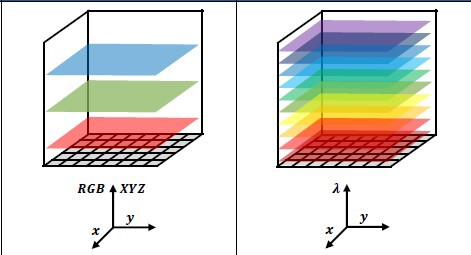
\includegraphics[height=2.5in]{figures/rgb_vs_hsi.jpeg}
\\
Las imágenes capturadas tienen la forma de "hipercubos"
\\
\url{https://towardsdatascience.com/what-are-hyper-spectral-images-a5de5d9fa91}
\\
\\
Estos espectros o bandas forman en su conjunto una especie de huella para cada pixel que permite reconocer materiales, diferentes tipos de vegetación, depósitos minerales o contaminantes.
\\
\\
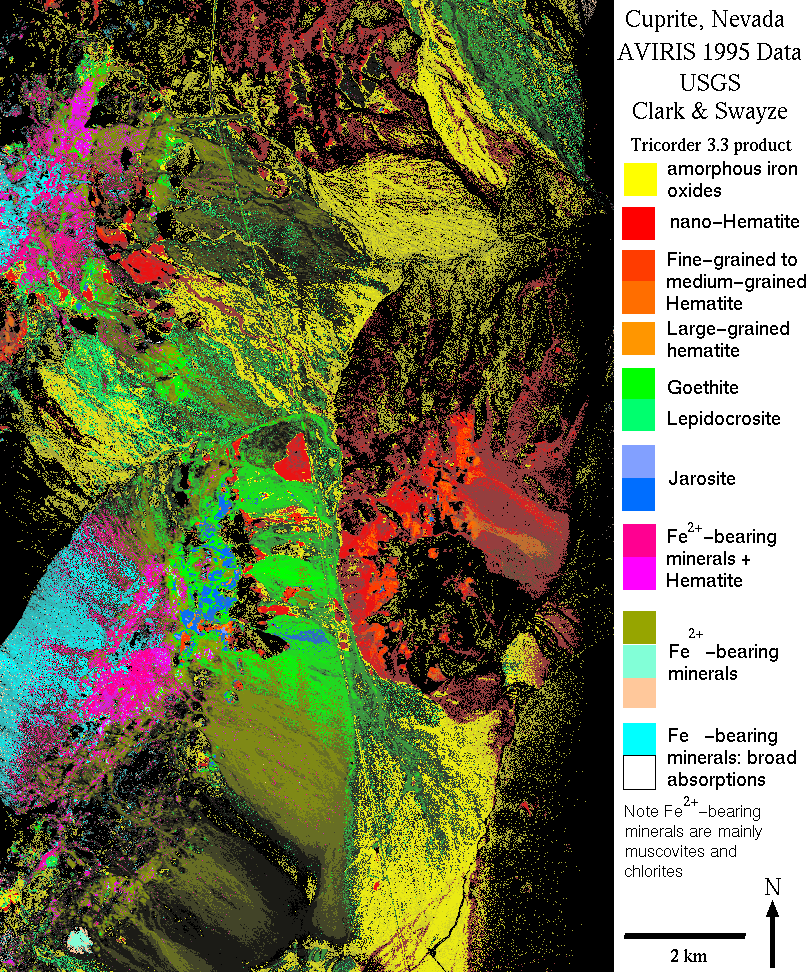
\includegraphics[height=2.5in]{figures/cuprite.png}
\\
En la imagen se puede observar como al cotejar las imágenes hiperespectrales con huellas de minerales estos pueden ser detectados sobre la corteza terrestre.
\\
\url{https://www.researchgate.net/figure/USGS-map-showing-the-location-of-different-minerals-in-the-Cuprite-mining-district-in_fig5_263532555}
\\
\\
En este tipo de imágenes podemos hablar de tres tipos de resoluciones: espacial, temporal y espectral, siendo esta última única en este tipo de cámaras. Local se refiere a la cantidad de metros cubiertos por cada pixel, por lo que para una misma cámara podrá cambiar de una imagen a otra. Resolución temporal se refiere a la cantidad de imágenes que es capaz de tomar una cámara por unidad de tiempo, por lo que será principalmente relevante en el momento de captura de la foto. La última resolución, la espectral, se refiere a la separación entre diferentes longitudes de onda medidos en un rango determinado, es decir cuantas mas bandas capturadas en un rango menor, mayor será la resolución espectral.
\\
\\
Conforme al avance de la tecnología, estas 3 resoluciones siguen aumentando realzando la necesidad de sistemas de procesado acorde.

\section{Reconfigurable hardware}
Las FPGA (de sus siglas en inglés, field programmable gate arrays) son chips basados en una matriz de bloques configurables llamada CLB (del ingles, configurable logic block) interconectados a su vez por una red también configurable.
\\
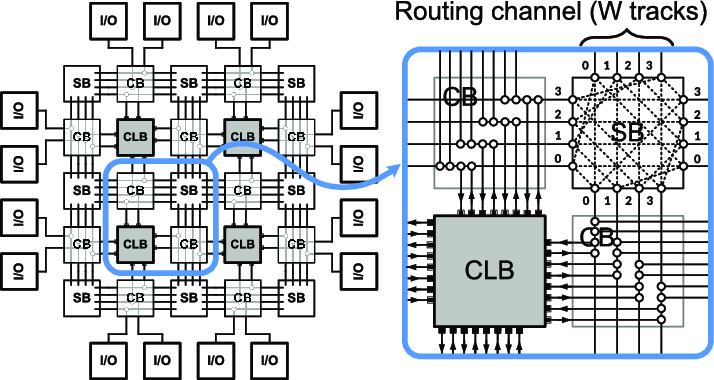
\includegraphics[height=2.5in]{figures/clb.png}
\\
Un CLB
\\
\url{https://www.researchgate.net/figure/Island-style-global-FPGA-architecture-A-unit-tile-consists-of-Configurable-Logic-Block_fig6_323820898}
\\
Al contrario que sistemas de propósito general como CPUs o GPUs, está arquitectura permite diseñar algoritmos con anchos de calculo arbitrarios, lo que resulta en muy buen rendimiento a la hora de procesar imágenes, tanto energético como temporal.
\\
\\
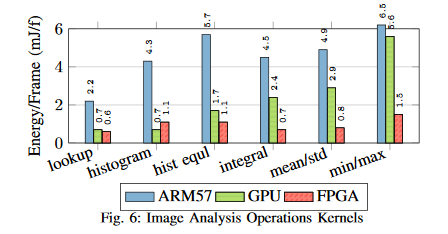
\includegraphics[height=2.5in]{figures/op_watt.png}
\\
ejemplo de operación por watt
\\
\url{https://arxiv.org/pdf/1906.11879.pdf}
\\
\\
\\
El entorno espacial no solo limita las capacidades energéticas, también presenta un desafío de cara a la radiación ionizante. Al ser este uno de los mercados objetivo de los fabricantes de FPGA, existen numerosos chips con las certificaciones de resistencia a radiación necesarias.
\\
Las ASICs proporcionan la misma flexibilidad que las FPGA a la hora del diseño pero su rigidez a la hora de fabricación les permite lograr un mejor rendimiento al solo incluir la lógica especifica del diseño, sin embargo, su coste en provectos de pequeña a mediana escala resulta prohibitivo. Además, la flexibilidad de las FPGA permite la reconfiguración ya en la nave, permitiendo el uso de diferentes algoritmos o el parcheo de bugs.
\\
\\
Además, puesto que la mayoría de algoritmos comparten ciertas operaciones básicas como pueden ser almacenamiento u operaciones matemáticas de precisión alta, los fabricantes de FPGA incluyen ciertos bloques prefabricados en el circuito, que aunque quitan cierta flexibilidad proporcionan mejor rendimiento que la misma lógica en CLBs. Estos bloques son principalmente memorias RAM y DSPs que permiten variedad de operaciones, entre ellas multiplicaciones o acumulaciones. Así se permite implementar algoritmos de alto rendimiento donde sería imposible usando solo lógica y acercan las FPGA un poco al ámbito de las ASIC.
\\
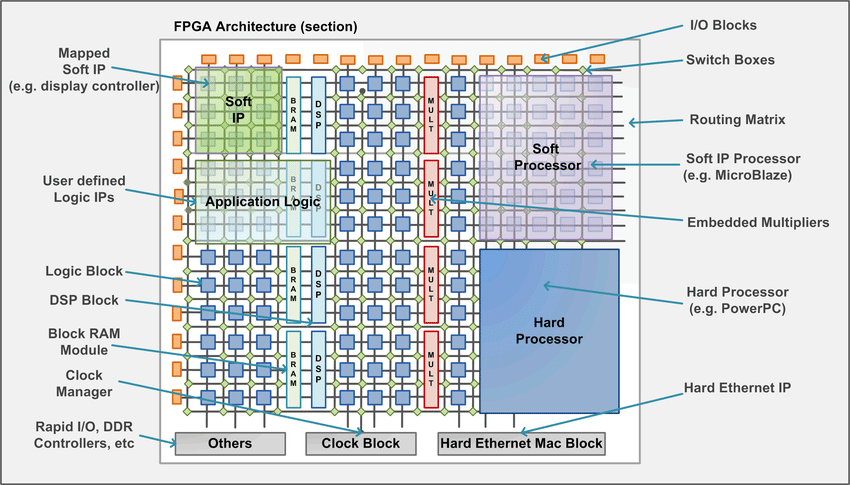
\includegraphics[height=2.5in]{figures/FPGA_heterogenea.png}
\\
Arquitectura heterogénea de una FPGA moderna
\\
\url{https://www.researchgate.net/figure/Heterogeneous-FPGA-platform-depicting-general-configurable-resources-hard-blocks-and_fig2_265125404}


\section{Anomaly detection}
QUIZÁS DEBO HABLAR DE OTROS TIPOS DE ALGORITMOS U OTROS ALGORITMOS DE ANOMALÍAS, O AMBOS
\\
\\
\\

La cantidad de datos que contienen estas imágenes y su gran variedad de usos da lugar a muchos tipos de algoritmos diferentes.
\\
\url{https://www.hindawi.com/journals/jece/2013/908906/}

La detección de anomalías es un tipo especial de técnicas de detección de objetivos sin información previa de los objetivos. El principal objetivo de este tipo de algoritmos es la detección de valores atípicos dentro de un conjunto de datos. La principal ventaja es que al no necesitar información previa de los objetivos tampoco son necesarias correcciones atmosféricas o radiometricas de ningún tipo.


\section{Project plan}
Primero se realizará una implementación del algoritmo en software en punto flotante que será validada con programas comerciales como ENVI o Spectral Python. Sobre esta base se diseccionarán los algoritmos para poder estudiarlos y acercarlos en la medida de lo posible a su implementación en hardware.
\\
A la vez, se estudiará la posible conversión de estas operaciones a punto fijo para lograr un mayor aprovechamiento de la lógica de la FPGA, en especial de los DSP. Además, el uso de DSP por operación es dependiente de la precision de los operandos[referencia a la tabla posterior]. Es necesario prestar especial detalle para poder minimizar los errores lo máximo posible sin exceder la capacidad del chip. Con este estudio hecho, se procederá a implementar la lógica en punto fijo y comparar los resultados de las dos implementaciones.


\section{RX algorithm}
Dentro de la detección de anomalías, el algoritmo RX es el mas usado y es conocido como el benchmark de este tipo de algoritmos.
Los algoritmos de detección de anomalías extraen los objetivos, es decir pixeles o regiones, que sean espectralmente distintos a sus circundantes o al conjunto de datos completo. Para que estos algoritmos sean efectivos, las anomalías deben ser lo suficientemente pequeñas relativamente al fondo. Estos algoritmos tienen la ventaja de no requerir información previa de los objetivos ni compensación por la refracción atmosférica. Además, los errores que pueda haber en la imagen no afectan a la detección de anomalías reales (creo que la mayor parte de esto ya lo he dicho arriba)
\bigskip
El algoritmo esta definido por la siguiente expresión:
\\
\[\delta ^{RX}(x) = (x-\mu)^{T}K^{-1}(x-\mu)\]

Donde $x$ es un pixel hiperespectral (un vector de tamaño igual al número de bandas), $\mu$ es la media de cada banda y $K$ es la matriz de covarianzass. Es importante decir que los resultados generados por el algoritmo son imágenes en escala de grises. Las anomalías poseen un valor alto, así, la primera anomalía corresponde con el pixel con el valor más alto, y sucesivamente.

El algoritmo está compuesto por lo tanto por los siguientes pasos:
\begin{itemize}
\item Calcular la media, la deviación y la covarianza K de la imagen
\item Calcular $K^{-1}$ es decir, la inversa de la covarianza
\item Calcular $\delta ^{RX}$ para cada pixel de la imagen
\item Ordenar los resultados
\end{itemize}

La fuente de esto es Molero2011.
